%!TEX root = report.tex

\newcommand{\q}[1]{``#1''}

\newcommand{\code}[1]{\textbf{\texttt{\uppercase{#1}}}}
\newcommand{\codeu}[1]{\textbf{\code{#1}}}

\newcommand{\inputAllPatterns}[1]{%
	\subsection{Client-Server}
\begin{figure}[H]
\centering
\includegraphics[scale=0.7]{6-evaluation/images/clientserver_frm.png}
\caption{Force Resolution Map for Client-Server pattern}
\label{fig:clientserver-frm}
\end{figure}
For the Client-Server pattern, the portability of the system increases, because the client and server (daemon) can be located on completely different systems.

The security has a slight negative impact because for communication between the client and server to be possible, the client and server have to expose an interface, which has to be secured. 

Reliability also has a small negative impact, because the communication between client and server relies on underlying communication infrastructure that could fail. 


	\section{Layers}
\label{sec:layers-pattern}
% see https://www.docker.com/sites/default/files/what-is-vm-diagram.png
Layers pattern is a architectural pattern that consists of several layers, which
each layer provides a set of services to the layer above and uses the services
of the layer below. Docker implements this pattern to separate the concerns of
each component with independent functionalities. Layers pattern implementation
of Docker, based on our investigation, is shown in Figure \ref{fig:layers-pattern}.
% \newglossaryentry{OS}{name=OS, description={Operating System}}

\begin{figure}[H]
\centering
\includegraphics[scale=0.5]{5-patterns/images/LayersPattern.png}
\caption{A layered overview of the Docker.}
\label{fig:layers-pattern}
\end{figure}

\begin{patdescription}
\item [Traceability]
Layers is implicitly mentioned in the Docker architecture in the online
documentation, specifically in the \textit{What is Docker’s architecture?}
section \cite{dockerarchi}.

\item [Source]
%TODO joris: there should be a standard way or referencing the page using the \cite command
Architectural patterns revisited -- a pattern language, P. 29
\cite{avgeriou2005architectural}

\item [Issue]
Docker provides several features (e.g. hosting the image, creating image, running container, and daemon supervision). Each of the features vary in terms of the functionality they give. Single implementation of features will certainly result in abundant usage of resources, because hosting the image means there must be huge amount of disk space available.
%TODO joris: Rephrase sentence about the hosting of the image. Rephrase, make clear why.
%
Overlapping may also occur since multiple Docker instances may use the same image or configuration file, which could be stored and organized elsewhere. Docker also has several dependencies, especially the Linux kernel components (\texttt{namespaces} and \texttt{cgroups}) for OS level virtualization.
Furthermore, Docker mostly needs remote supervision or control, since Docker usually runs in the cloud. Therefore, the features must be separated into several independent components and their dependencies and communication have to be clearly separated and maintained.

\item [Assumptions/Constraints]
%TODO joris: improve and correct this
 Docker is able to run only in Linux kernel since it uses \codeu{namespaces} and \codeu{cgroups} technology, which is only available in Linux kernel. However, Docker is also possible to be run on other OS although using virtual machine. The connection between local and remote components are carried out through secured TCP/IP connection. 

\item [Solution]
Docker is separated into several components that have their own functionality, as can be seen in Figure \ref{fig:layers-pattern}. The main components are:
\begin{itemize}
    \item Containers
    \item Docker daemon
    \item Local Docker client
    \item Libcontainer
    \item Linux kernel
\end{itemize}

Everything inside the dotted box is located on the same host. Inter-process communication is utilized to communicate between Docker, containers, libcontainer, and Linux kernel components, but Docker daemon, plugins, and Docker client communicate using Docker API
\footnote{\url{https://github.com/docker/docker/blob/master/api/common.go}}. Remote connections are managed through secured TCP/IP based connection.

\item [Rationale] 
Layers are very good in terms of sharing and reusability. In this way, several Docker daemon that uses the same image can just fetch it through the Docker registry. Using Docker registry also reduce disk space for storing images and increase easiness of sharing images. Layers pattern also supports connection to other layer, such as connection to plugins. It is also manageable to supervise remote Docker daemon through remote Docker client.

\item [Implications] 
This pattern gives positive implication to portability as clear separation of containers, Docker daemon, Docker registry, and Docker client makes Docker portable. Utilizing Docker registry also promotes sharing images, which make it easier to deploy an application without knowing what platform running below it.\\
A host is open to public in the communication of Docker daemon and Docker registry and remote client. This pattern provides the ability to secure all the communication from single place. This can increase the security, because focus on security is reduces to single place, meaning that strengthening the security there makes everything more secure. \\ 
However, a security breach will effect the entire system and not only a single component. This security layer can be easily replicated, having a positive impact on reliability. The security is defined in a single place, and so the level of security that is defined there can be expected from each component. 

\item [Related Patterns]
\begin{mynesteditemlist}
	\item Client-server
	\item Shared repository
\end{mynesteditemlist}

\end{patdescription}

% \clearpage



	\section{Shared/Active repository}
%\textit{Can we consider the docker registry a shared repository?}
% Schemas
%http://fr.slideshare.net/Docker/https-dldropboxusercontentcomu20637798docker-meetup-freiburg
% http://blog.octo.com/en/docker-registry-first-steps/   http://fr.slideshare.net/egorpushkin/docker-demo   
% Because of Pull/¨Push can we talk about Pattern publish suscribe ?   Asynhcronous Queuing ?
 \begin{figure}[H]
 \centering
 \includegraphics[scale=0.55]{5-patterns/images/SharedRepo.png}
 \caption{The shared repository with brokered authentication}
 \label{fig:docker-registry}
 \end{figure}
Using the Docker files and the docker commands, personalized images can be created that support a specified project. Docker allows these images to be stored in a docker registry, earlier discussed in subsection \ref{subsec:dockerregistry}. Anyone with access to this registry can pull this image and use it.\\
Users of the application a specific project provides, are able to pull the image. This allows running the application, thereby obtain the desired functionality. The registry also allows the image to be easily shared with other developers working on any related project.\\
This makes the docker registry a shared repository.
%TODO joris: add concluding sentence: 'So because the image can be easily shared, it increases porta/mainta/sec... enz.


%TODO joris: is this relevant? not specific to the pattern, should be discussed in logical view or earlier?
% Docker itself hosts a few registries that can be used called ``DockerHub'' \cite{} and ``Docker Trusted''. 
%Two alternatives exist:DockerHub and Docker Trusted Registry. \\
The Docker registry also contains functionality for sending notifications when certain events occur \cite{docknotif}. This makes the docker registry an active repository as well.

\begin{patdescription}
\item[Traceability]
The Shared Repository pattern can be deducted from the online documentation : \cite{dockregistry} ``The Registry is a stateless, highly scalable server side application that \textbf{stores} and lets you \textbf{distribute} Docker images. A registry is a storage and content delivery system.''
Everything dealing with the registry is in the "Registry folder" in the Docker repository.

% File store.go , registry.go

\item[Source]
Patterns of Enterprise Application Architecture, P.322 \cite{eaa}\\
Architectural Patterns Revisited - A Pattern Language, P.13 \cite{avgeriou2005architectural}\\
Pattern-oriented Software Architecture - Volume 4, P.202 \cite{wiley4}

\item[Issue]
Docker provided a way for the user to control the storage and distribution of images. \\
The user wants to be alerted of new events happening in the registry through notifications. % Develop ?

%\item[Assumptions/ Constraint]

\item[Solution] %how does it work ?
Users interact with a registry by using docker push and pull commands. % develop

\item[Rationale] % in which way this pattern helps Docker? What is the goal ? KD
 After the integration of the Shared Repository Pattern each has one central repository containing their images and they can it access using a loggin.
 Users can also access images from others users : The registry is a sharing unit. \\
 
 \item [Implications]
Users can get their own images from the public registry and also the ones created by other users. % share
The use of this pattern enhances Reusability, Changeability, Maintainability, Integrability because the Registry is central.

\item [Related Patterns]
Publish Subscribe 
Brokered Authentication

\textit{Users can share and distribute images in the Docker Registry.}
 
\end{patdescription}


	\section{Publish Subscribe}
% Deisgn Pattern : Event driven messaging 
\begin{patdescription}

\item[Traceability]
The notification mechanism of the Docker Registry uses the Publish Subscribe Pattern \cite{docknotif}.

\item[Source]
Pattern Oriented Software Architecture- Volume 1
%http://soapatterns.org/designpatterns/eventdrivenmessaging

\item[Issue] The user wants to be alerted about certain events/changes that occur in a registry.
The notification system needs a mechanism in order to send those events to the user.

\item[Assumptions/Constraints] 
This pattern is used at a lower level in the Docker Registry/Active Repository Pattern.



\item[Solution]

\item[Rationale] 

%TODO fix, remove the big quote. Use POSA or something

\begin{quote}
"Notifications are sent to endpoints via HTTP requests. Each configured endpoint has isolated queues, retry configuration and http targets within each instance of a registry. When an action happens within the registry, it is converted into an event which is dropped into an inmemory queue. When the event reaches the end of the queue, an http request is made to the endpoint until the request succeeds. The events are sent serially to each endpoint but order is not guaranteed."% it seems like it's the way it works
\end{quote} 

\item[Implications] %After the integration of the Publish-Suscribe pattern BLABLABLA
The Publish Suscribe Pattern enhances Integrability,Modifiability because publisher and suscribers aren't directly connected.% develop

\item [Related Patterns]
Shared/Active Repository Pattern


\end{patdescription}

\begin{figure}[H]
\centering
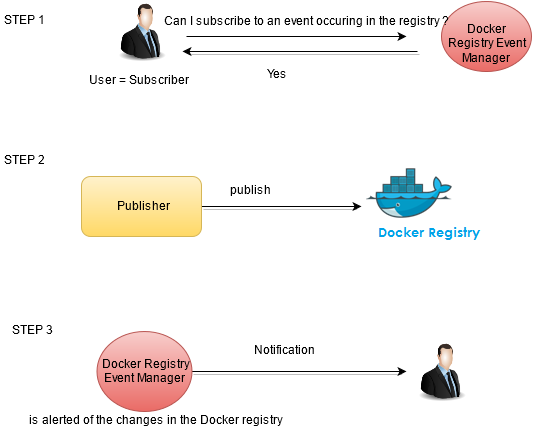
\includegraphics[scale=0.7]{5-patterns/images/RegistryPS.png}
\caption{Events managing- Publish Subscribe Pattern}
\label{fig:publish-subscribe}
\end{figure}


	% !TEX root = ../report.tex
\subsection{Brokered Authentication}

\begin{figure}[H]
\centering
\includegraphics[scale=0.7]{6-evaluation/images/brokered_auth_frm.png}
\caption{Force Resolution Map for Brokered Authentication pattern.}
\label{fig:brokered-auth-frm}
\end{figure}

The use of this pattern increases the portability, because the authentication service is decoupled from the registry. The authentication service can run on a completely different system. 

Reliability is ensured because if the user cannot push/pull, an error message is
prompt. In that way, the user is notified in case of a failure in his
authentication. (see definition of Reliability in the Shared Repository Pattern
evaluation).

However, there is also a drawback in the reliability, because the centralized
authorization service can be a single point of failure. It must be online
and available, otherwise the client cannot get his token. If the brokered
authentication becomes unavailable, the registry and the client cannot
communicate with each other. Redundant and back-up authentication brokers are the
example solutions of this problem.

Security is ensured because the registry and the client do not communicate
directly. The Bearer token is a barrier of protection between the two
components. However, security tokens must be signed by the authentication broker.
If they are not, their integrity cannot be verified. This could result in
attackers trying to issue false tokens.

Figure \ref{fig:brokered-auth-frm} concludes the contribution of this pattern.

	% !TEX root = ../report.tex
\section{Plugin}
\label{sec:pattern-plugin}
Plugin pattern basically expands the capability of a particular software. Plugin
pattern also provides centralized, runtime configuration\cite{eaa}. An
illustration of plugin pattern is shown in Figure \ref{fig:plugin-pattern}.

\begin{figure}[H]
\centering
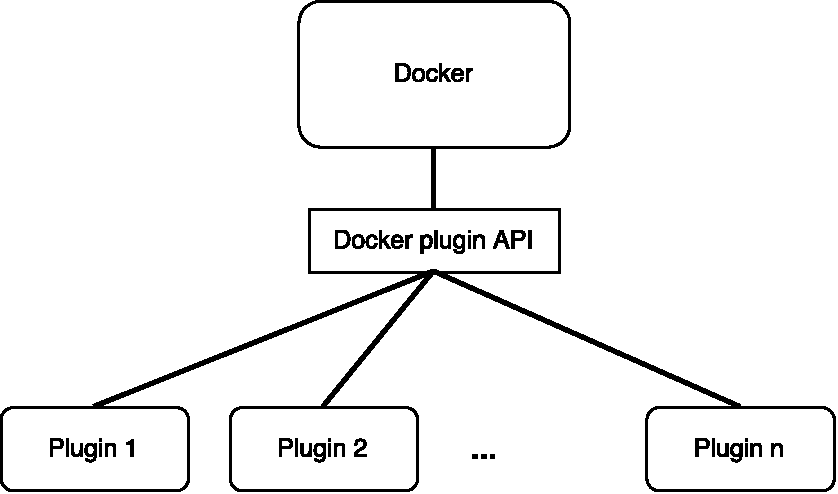
\includegraphics[scale=0.5]{5-patterns/images/plugins-pattern.pdf}
\caption{Plugin pattern illustration for Docker.}
\label{fig:plugin-pattern}
\end{figure}

\begin{patdescription}

\item [Traceability]
The existence of Docker plugin becomes apparent from its documentation, which
describes the plugin feature of Docker \cite{dockerplugindocs}.

Additionally, the directories \verb|docker/pkg/plugin/|\footnote{\url{https://github.com/docker/docker/tree/master/pkg/plugin}} and
\verb|docker/daemon/graphdriver/plugin.go|\footnote{
\url{https://github.com/docker/docker/blob/master/daemon/graphdriver/plugin.go}}
(among others) in the project's repository contain the code for discovering
plugin and the interfaces the plugin should implement.

\item [Source]
Patterns of Enterprise Application Architecture, P. 499 \cite{eaa}

\item [Issue]
%TODO joris: make neat sentence
Several of Docker users desired functionalities are not natively provided by
docker. Docker provides the mechanism so that third party custom-built tools
that provide this missing functionality to extend Docker. These customizations
mean that third party developers are able to write tools, extending Docker's
core functionality\cite{dockerpluginblog}. The additional functionality that is
added, is only usable during run time.
%TODO joris: add consequences of this issue (regarding key d's?).


\item [Assumptions/Constraints]
\begin{mynesteditemlist}
\item plugin can only extend the functionality of the Docker components if
necessary APIs are provided for certain need or use.
\end{mynesteditemlist}

\item [Solution]
Docker implements the plugin pattern to link several Docker's extendable component's interfaces with third-party code at runtime.

\item [Rationale]  % https://docs.docker.com/engine/extend/plugin_api/
By using plugin pattern, any feature that is currently not supported natively
by Docker can be added. The users can also develop a custom code that will
exploit Docker APIs to fulfill their need.

\item [Implications]
The use of the plugin pattern means that the adaptability increases, because
plugin allow the application to be adapted with new features. For the security
concern, it means that there is extra communication over the API which has to be
secured. The security of the plugin themselves cannot be guaranteed by Docker.

\item [Related Patterns]
\begin{mynesteditemlist}
\item Broker
\end{mynesteditemlist}
\end{patdescription}


	% !TEX root = ../report.tex
\section{Broker}
\manuallabel{pattern:broker}{Broker}
\begin{figure}[H]
\centering
\includegraphics[scale=0.43]{5-patterns/images/broker.png}
\caption{Broker for communication between Docker daemon and a plugin.}
\label{fig:broker-pattern}
\end{figure}

\begin{patdescription}
\item [Traceability]
The use of the Broker pattern can be found in the proxy package in the source code:\\
\verb| docker/pkg/proxy/tcp_proxy.go|\footnote{\url{https://github.com/docker/docker/blob/master/pkg/proxy/tcp_proxy.go}}.

\item [Source]
Pattern-oriented Software Architecture - Volume 4, P.237 \cite{wiley4} \\
Architectural Pattern Revisited - A Pattern Language, P.34 \cite{avgeriou2005architectural}

\item [Issue]
Docker consists of multiple processes. For example, the client and daemon are separate processes and also the plugins are separate processes.

These processes have to communicate with each other. However, dealing with the challenges of inter-process communication in the application code would greatly increase the complexity.
The application components should be shielded form the details of the inter-process communication.

\item [Assumptions/Constraints]
\begin{mynesteditemlist}
\item All the communication between the components in different processes have to go via the Broker.
\end{mynesteditemlist}

\item [Solution]
Use a Broker to separate the logic for communication between the processes from the application functionality. Use a component-based model (using Proxies) to allow local components to invoke methods on components in remote processes as if they were local.

\item [Rationale]  
The Broker pattern allows for and handles all the communication between the different processes. 

This means that the logic for inter-process communication does not have to be implemented on a per-component basis.

\item [Implications]
Using the Broker pattern is good for the portability, because it does not matter if a component is part of a different process (running locally or remotely).

This pattern is also good for the security, since the Broker is a single entry point for all the inter-process communication, which makes it easier to secure. This has been done by using Transport Layer Security for the communication between the processes.

Additionally, the interoperability (compatibility) is increased, because it becomes possible for two components (in two different processes) to exchange information. 

The Broker does however introduce a performance overhead, which decreases the performance efficiency.

%TODO: reliability??

%TODO: what about portability??

\item [Related Patterns]
\begin{mynesteditemlist}
\item Plugin
\item Proxy
\item Client-Server
\end{mynesteditemlist}

\end{patdescription}

}
%\subsection{Client-Server}
\begin{figure}[H]
\centering
\includegraphics[scale=0.7]{6-evaluation/images/clientserver_frm.png}
\caption{Force Resolution Map for Client-Server pattern}
\label{fig:clientserver-frm}
\end{figure}
For the Client-Server pattern, the portability of the system increases, because the client and server (daemon) can be located on completely different systems.

The security has a slight negative impact because for communication between the client and server to be possible, the client and server have to expose an interface, which has to be secured. 

Reliability also has a small negative impact, because the communication between client and server relies on underlying communication infrastructure that could fail. 


%\subsection{Layers}

\begin{figure}[H]
\centering
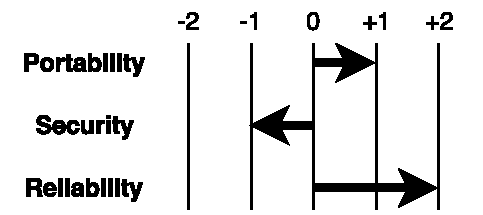
\includegraphics[scale=0.7]{6-evaluation/images/layers_frm.pdf}
\caption{Force Resolution Map for Layers pattern.}
\label{fig:layers-frm}
\end{figure}

This pattern gives positive implication to portability as clear separation of
containers, Docker daemon, Docker registry, and Docker client makes Docker
portable and loosely coupled. Utilizing Docker registry also promotes sharing
images, which make it easier to deploy an application without knowing what
platform running below it. Exposing TCP/IP connection, specifically REST,
contributes to negative effect on the security. It means that any unwanted
connections or attacks could possible exploit this hole. However, this weak
point is compensated by other patterns. 

Furthermore, decoupling some components
means that the components below or above can be replicated in order to gain more
reliability as it has more availability. Thus, this patterns give positive
effect to the reliability. 

The summary of the Layers pattern evaluation is shown
in FRM in Figure \ref{fig:layers-frm}.


%\subsection{Plugin}
\begin{figure}[H]
\centering
\includegraphics[scale=0.7]{6-evaluation/images/plugin_frm.png}
\caption{Force Resolution Map for Plugin pattern}
\label{fig:plugin-frm}
\end{figure}
The Plugin pattern greatly increases the portability, because it increases the adaptability by allowing third parties to develop extensions for Docker. 

It has a slight negative impact on the security, because there is communication between the daemon and plugin process which has to be secured. Additionally, the security of the plugins is not controlled by Docker, so defects in a plugins security can affect the security of the Docker daemon as well. 

There are no significant impacts on the reliability because of this pattern.


%\subsection{Broker}
\begin{figure}[H]
\centering
\includegraphics[scale=0.7]{6-evaluation/images/broker_frm.png}
\caption{Force Resolution Map for Broker pattern}
\label{fig:broker-frm}
\end{figure}
The use of the Broker pattern is very beneficial for the portability, because it allows the use of components in different processes, potentially running on different machines.

This pattern is also positive for the security of Docker, because it is a single entrypoint for all inter-process communication, which is easier to secure than multiple entrypoints.

%TODO: reliability


%\subsection{Proxy}
\begin{figure}[H]
\centering
\includegraphics[scale=0.7]{6-evaluation/images/proxy_frm.png}
\caption{Force Resolution Map for Proxy pattern}
\label{fig:proxy-frm}
\end{figure}
The use of the Proxy pattern has a positive impact on the portability, because the location of the component accessed through the proxy is transparent for the caller.
There is a small negative impact on security, because the invocation on the Proxy are forwarded to the component in another process. This communication has to be secured.



%% !TEX root = ../report.tex
\subsection{Shared/Active repository} 

\begin{figure}[H]
\centering
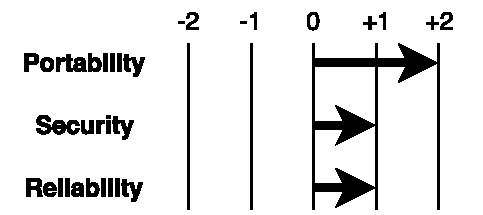
\includegraphics[scale=0.7]{6-evaluation/images/shared_active_repo_frm.pdf}
\caption{Force Resolution Map for Shared/Active Repository pattern.}
\label{fig:shared-active-repo-frm}
\end{figure}

According to Wikipedia, a reliable service is one that notifies the user if
delivery fails, while an ``unreliable'' one does not notify the user if delivery
fails. Based on this definition we can consider that the registry is reliable
because in case a push command doesn't work the user is notified (same system as
Github for example) by an error message/prompt and can try again.

Security is enhanced because the access to the registry is controlled by a login
and passwords for the users. Moreover, the push and pull commands in the
registry are also secure (see Brokered Authentication Pattern).

The docker registry is good for portability because whatever the environment of
the user everybody can subscribe and access this functionality.

The Shared Repository pattern has effects on other quality attributes such as
integrability, modifiability and re-usability. Figure \ref{fig:shared-active-repo-frm}
shows the FRM of Shared/Active Repository pattern.

%\input{6-evaluation/Publish_Suscribe.tex}

\newcommand{\todonote}[1]{\textcolor{red}{#1}}
\newcommand{\attention}[1]{\textcolor{green}{#1}}
\newcommand{\HRule}{\rule{\linewidth}{0.5mm}}
\newcommand{\cellBox}[1]{\pbox{0.6\textwidth}{#1}}
%\newcommand\myworries[1]{\textcolor{red}{#1}}
\newcommand\myworries[1]{}

\newcommand{\ign}[1]{}

% Commands for rotating table header
\newcommand*\rot{\rotatebox{90}}
\newcommand*\OK{\ding{51}}

\newcommand{\compactCell}[1]{%
    \adjustbox{valign=t}{%
        \begin{minipage}{\linewidth}%
            #1%
        \end{minipage}%
    }%
}

\newcommand{\compactList}[2]{%
    %\begin{minipage}[t][][p]{\linewidth}%
    %\begin{minipage}{\linewidth}%
    \adjustbox{valign=t}{%
        \begin{minipage}{\linewidth}
            \begin{#1}[%
                nosep,
                nolistsep,
                topsep=1pt,
                partopsep=0pt,
                parsep=0pt,
                %itemsep=0pt,
                itemindent=0pt,
                %labelsep=*,
                %align=margin,
                align=left,
                %leftmargin=\linewidth,
                leftmargin=*,
                labelwidth=*,
                after=\strut,
                ]#2\end{#1}%
        \end{minipage}%
    }%\end{adjustbox}
}%

\newcommand{\allotOfText}{%
    LaTeX styled as LATEX, and a shortening of Lamport TeX is a word processor and a document markup language. It is distinguished from typical word processors such as Microsoft Word and Apple Pages in that the writer uses plain text as opposed to formatted text, relying on markup tagging conventions to define the general structure of a document (such as article, book, and letter), to stylise text throughout a document (such as bold and italic), and to add citations and cross-referencing. A TeX distribution such as TeXlive or MikTeX is used to produce an output file (such as PDF or DVI) suitable for printing or digital distribution.
}
%
%\newcolumntype{R}[2]{%
%    >{\adjustbox{angle=#1,lap=\width-(#2)}\bgroup}%
%    l%
%    <{\egroup}%
%}
%\newcommand*\rotmc{\multicolumn{1}{R{90}{1em}}}% no optional argument here, please!
%

%\newcolumntype{R}[2]{%
%    >{\adjustbox{angle=#1,lap=\width-(#2)}\bgroup}%
%    l%
%    <{\egroup}%
%}
%\newcommand*\rot{\multicolumn{1}{R{90}{1em}}}% no optional argument here, please!


%command to decrease the size it takes to write
%L{0.5\textwidth}. This will now be:
%L{\tw{0.5}}. A small difference, but it adds up
\newcommand{\tw}[1]{#1\textwidth}

\newcommand\crule[3][black]{\textcolor{#1}{\rule{#2}{#3}}}


\newcommand{\getNr}[1]{%
    \getNext{#1}
    \arabic{#1}
}

\makeatletter

%manually lable something
%like \manuallabel{fr:01}{The first }
% \ref{fr:01} will then hold "The first req"
\newcommand{\manuallabel}[2]{\def\@currentlabel{#2}\label{#1}}

\newcommand{\getNext}[1]{%
    %check if counter with that name excists
    \@ifundefined{c@#1}
    {% the counter doesn't exist
        \newcounter{#1}\setcounter{#1}{1}%
    }
    {% the counter exists
        \stepcounter{#1}%
    }%
}
\newcommand{\nextNrRef}[1]{%
\getNext{#1}
\manuallabel{#1:\arabic{#1}}
{\uppercase{#1}-\arabic{#1}}
\arabic{#1}
}


\newcommand{\req}[1]{%
    \uppercase{#1}-\nextNrRef{#1}
}

\newcommand{\frReqRowNoRule}[3]{%
    \phantomsection
    \getNext{FR}
    \manuallabel{fr:#1}{FR-\arabic{FR}} 	
    FR-\arabic{FR} &
    \ifcase\pdfstrcmp{#2}{Must}%
    \textbf{#2}
    \else
    #2
    \fi
    &
    #3
    \\

}

\newcommand{\frReqRow}[3]{%
    \midrule
    \frReqRowNoRule{#1}{#2}{#3}
}	

\newcommand{\newshortlabel}[2]{\phantomsection\getNext{#1}\manuallabel{#1:#2}{\uppercase{#1}-\arabic{#1}}\uppercase{#1}-\arabic{#1}}

\newcommand{\nsl}[2]{\newshortlabel{#1}{#2}}


\newcommand{\hlReqRow}[4]{%
    \midrule
    \\
    \phantomsection
    \req{HL} &
    \ifcase\pdfstrcmp{#2}{Must}%
    \textbf{#2}
    \else
    #2
    \fi
    & \textbf{#3} \\
    & & #4
    \\
    \\
}

\newcommand{\reqRow}[4]{%
    \midrule
    \phantomsection
    \req{#1}
    \manuallabel{#1:#2}{\uppercase{#1}-\arabic{#1}} &
    \ifcase\pdfstrcmp{#3}{Must}%
    \textbf{#3}
    \else
    #3
    \fi
    &
    #4
    \\
}		

\newcommand{\risk}[7]{%
    \begin{table}[H]
        \begin{tabular}{L{0.3\textwidth} L{0.7\textwidth}}\toprule\phantomsection\getNext{#1-RISK}\manuallabel{#7}{#1-RISK\arabic{#1-RISK}}\textbf{#1-RISK\arabic{#1-RISK}} & \textbf{#2} \\*
            \midrule
            \textbf{Probability of occurrence} & #3 \\*
            \midrule
            \textbf{Consequences}              & #4 \\*
            \midrule
            \textbf{Prevention}                & #5 \\*
            \midrule
            \textbf{Reaction}                  & #6 \\*
            \bottomrule
        \end{tabular}
        \caption{#1-RISK\arabic{#1-RISK} -- #2}
    \end{table}
    \vspace{0.5cm}
}

\newcommand{\pattern}[1]{%
	{\fontfamily{qcr}\selectfont\uppercase{#1}}}

\makeatother


%\makeatletter
%\newcommand{\req}[1]{%
%	\newcommand{\curCountVal}{\arabic{\getNr{#1}}}
%	\label{\curCountVal}
%}
%\makeatother

%	\label{#1:\arabic{#1}}
%	\arabic{#1}

% Glossary macros
\newcommand{\qos}{Quality of Service\xspace}
